\section{Обработка событий}
\label{sec:events}

Для того чтобы создать программу взаимодействующую с пользователем необходимо 
обрабатывать события произошедшие в графическом окне. Следующие события 
обрабатываются библиотекой \code{Graphics}: нажатие на клавишу клавиатуры, на 
кнопку мыши и её перемещение.

Стиль и устройство программы изменяются: программа превращается в бесконечный 
цикл ожидающий события. После обработки нового события, программа вновь 
возвращается в бесконечный цикл, если только это он не было предвиденно для 
остановки программы.

\subsection{Тип и функции событий}
\label{subsec:types_and_functions_for_events}

Существует следующая главная функция ожидания события: \code{wait\_next\_event} 
с типом \type{list -> status}.

Различные события определены типом сумма \type{event}:

\begin{lstlisting}[language=OCaml]
type event = Button_down | Button_up | Key_pressed | Mouse_motion | Poll ;;
\end{lstlisting}

Первые четыре значения соответствуют нажатию и отпусканию кнопки мыши, нажатие 
на клавишу клавиатуры и перемещение мыши. Если конструктор \code{Poll} добавить 
в список событий, то ожидание не будет блокирующим. Функция возвращает значение 
типа \type{status}.

\begin{lstlisting}[language=OCaml]
type status = 
  { mouse_x : int;
    mouse_y : int;
    button : bool;
    keypressed : bool;
    key : char};;
\end{lstlisting}

Поля этой записи содержат координаты курсора мыши, булево значение равное истине 
если кнопка мыши была нажата, такое же значение для клавиатуры и последнее 
значение содержит символ нажатой клавиши. Следующие функции используют значения 
этой записи.

\begin{itemize}
	\item \code{mouse\_pos} : \type{unit -> int * int} : возвращает положение 
курсора на экране, если курсов вне графического окна, то координаты находятся 
вне окна.
	\item \code{button\_down} : \type{unit -> bool} : указывает на нажатие 
кнопки мыши 
	\item \code{read\_key} : \type{unit -> char} : возвращает символ нажатой 
клавиши
	\item \code{key\_pressed} : \type{unit -> bool} : указывает на нажатие 
клавиши клавиатуры, ожидание не блокирующее 
\end{itemize}

Библиотека \code{Graphics} обрабатывает события на минимальном уровне, однако 
полученный код переносим на различные платформы: Windows, MacOS или X-Windows. 
Именно по этой причине данная библиотека не различает кнопки мыши. На 
компьютерах Mac существует всего одна кнопка. Другие события, как закрытие окна 
или изменение размеров окна не доступны и оставлены на обработку библиотекой.

\subsection{Скелет программы}
\label{subsec:program_skeleton}

Все программы с пользовательским интерфейсом содержат цикл, потенциально 
бесконечный, осуществляющий ожидание событий от пользователя. Как только оно 
возникает, программа выполняет связанное с ним действие. У следующей функции 5 
функциональных аргументов. Первый и второй служат для запуска и остановки 
программы, два следующие это функции обрабатывающие события связанные с 
клавиатурой и мышью. Последний аргумент служит для управления исключениями, 
которые могут возникнуть во время вычислений. События, заканчивающие программу, 
возбуждают исключение \code{End}.

\begin{lstlisting}[language=OCaml]
# exception Fin;;
exception Fin
# let squel f_init f_end f_key f_mouse f_except = 
  f_init () ;
  try 
      while true do 
        try 
          let s = Graphics.wait_next_event 
                    [Graphics.Button_down; Graphics.Key_pressed] 
          in if s.Graphics.keypressed then f_key s.Graphics.key
             else if s.Graphics.button 
                  then f_mouse s.Graphics.mouse_x s.Graphics.mouse_y
        with 
             Fin -> raise Fin
           |  e  -> f_except e
      done
  with 
      Fin  -> f_end () ;;
val squel :
  (unit -> 'a) ->
  (unit -> unit) ->
  (char -> unit) -> (int -> int -> unit) -> (exn -> unit) -> unit = <fun>
\end{lstlisting}

Этот скелет мы используем в программе моделирующей печатную мини--машину. 
Нажатие на клавишу выводит соответствующий символ, нажатие на кнопку мыши меняет 
текущую позицию, а клавиша с символом \S заканчивает программу. Единственная 
трудность заключается в переходе на новую строку. Для упрощения, предположим что 
высота символа не превышает 12 пикселей.

\begin{lstlisting}[language=OCaml]
# let next_line () = 
   let (x,y) = Graphics.current_point() 
   in if y>12 then Graphics.moveto 0 (y-12)
      else Graphics.moveto 0 y ;;
val next_line : unit -> unit = <fun>
# let trait_char c = match c with 
     '§'  -> raise Fin
   | '\n' -> next_line ()
   | '\r' -> next_line ()
   |   _  -> Graphics.draw_char c ;;
val trait_char : char -> unit = <fun>
# let go () = squel 
   (fun () -> Graphics.clear_graph () ; 
              Graphics.moveto 0 (Graphics.size_y() -12) )
   (fun () -> Graphics.clear_graph())
   trait_char
   (fun x y -> Graphics.moveto x y)
   (fun e -> ()) ;;
val go : unit -> unit = <fun>
\end{lstlisting}

Клавиша \code{DEL}, стирающая предыдущий символ, не обрабатывается этой 
программой.

\subsection{Пример: telecran}
\label{subsec:example_telecran}

Telecran небольшая игра рисования для тренировки координации. При помощи клавиш 
контроля точка на планшете может передвигаться по X и Y не отрывая пера от 
планшета. При помощи данной модели, мы проиллюстрируем взаимодействие программы 
и пользователя. Для этого, применим предыдущий скелет, а также некоторые клавиши 
клавиатуры для указания движения.

Определим тип \type{state} --- запись в которой будет храниться размер планшета 
выраженный в количестве позиций по X и Y, текущая позиция пера, масштаб для 
просмотра, цвет которым рисует перо, цвет экрана и цвет для определения 
положения пера на экране.

\begin{lstlisting}[language=OCaml]
# type state = {maxx:int; maxy:int; mutable x : int; mutable y :int;
               scale:int;
               bc : Graphics.color;
               fc: Graphics.color; pc : Graphics.color};;
\end{lstlisting}

Функция \code{draw\_point} рисует точку по указанным координатам, масштабу и 
цвету.

\begin{lstlisting}[language=OCaml]
# let draw_point x y s c =
   Graphics.set_color c;
   Graphics.fill_rect (s*x) (s*y) s s;;
val draw_point : int -> int -> int -> Graphics.color -> unit = <fun>
\end{lstlisting}

Все функции инициализации, обработки событий и выхода из программы получают 
параметр соответствующий состоянию. Вот как определены первые четыре функции.

\begin{lstlisting}[language=OCaml]
# let t_init s () = 
   Graphics.open_graph (" " ^ (string_of_int (s.scale*s.maxx)) ^
     "x" ^ (string_of_int (s.scale*s.maxy)));
   Graphics.set_color s.bc;
   Graphics.fill_rect 0 0 (s.scale*s.maxx+1) (s.scale*s.maxy+1);
   draw_point s.x s.y s.scale s.pc;;
val t_init : state -> unit -> unit = <fun>
# let t_end s () = 
   Graphics.close_graph();
   print_string "Good bye..."; print_newline();;
val t_end : 'a -> unit -> unit = <fun>
# let t_mouse s x y = ();;
val t_mouse : 'a -> 'b -> 'c -> unit = <fun>
# let t_except s ex = ();;
val t_except : 'a -> 'b -> unit = <fun>
\end{lstlisting}

Функция \code{t\_init} открывает окно и выводит перо на текущую позицию, 
\code{t\_end} закрывает это окно и выводит сообщение, \code{t\_mouse} и 
\code{t\_except} ничего не делают. В этой программе действия мыши, так же как и 
исключения, не обрабатываются. Последние могут возникнуть во время запуска 
программы. Функция \code{t\_key} --- главная, она отвечает за обработку нажатий 
на клавиатуру.

\begin{lstlisting}[language=OCaml]
# let t_key s c = 
  draw_point s.x s.y s.scale s.fc;
   (match c with
   '8' -> if s.y < s.maxy then  s.y <- s.y + 1;  
 | '2' -> if s.y > 0 then s.y <- s.y - 1
 | '4' -> if s.x > 0 then s.x <- s.x - 1 
 | '6' -> if s.x < s.maxx then s.x <- s.x + 1 
 | 'c' ->   Graphics.set_color s.bc;
            Graphics.fill_rect 0 0 (s.scale*s.maxx+1) (s.scale*s.maxy+1); 
            Graphics.clear_graph()
 | 'e' -> raise End
 | _ -> ());
  draw_point s.x s.y s.scale s.pc;;
val t_key : state -> char -> unit = <fun>
\end{lstlisting}

Она закрашивает текущую точку цветом пера. В зависимости от переданного символа 
изменяет, если возможно, текущую позицию пера (символы '2','4','6','8'), очищает 
экран (символ 'c') или возбуждает исключение \code{End} (символ 'е'), затем 
выводит новое положение пера. Все остальные символы проигнорированы. Выбор 
клавиш для перемещение пера основывается на расположении клавиш малой цифровой 
клавиатуры.

И наконец, определим состояние, а также воспользуемся скелетом следующим 
образом:

\begin{lstlisting}[language=OCaml]
# let stel = {maxx=120; maxy=120; x=60; y=60; 
             scale=4; bc=Graphics.rgb 130 130 130;
             fc=Graphics.black; pc=Graphics.red};;
val stel : state =
  {maxx=120; maxy=120; x=60; y=60; scale=4; bc=8553090; fc=0; pc=16711680}
# let slate () = 
   skel (t_init stel)  (t_end stel) (t_key stel) 
    (t_mouse stel) (t_except stel);;
val slate : unit -> unit = <fun>
\end{lstlisting}

Вызов функции \code{slate} выводит на экран окно и ожидает действий с 
клавиатуры. На рисунке \ref{fig:telecran} приведено изображение, реализованное 
этой программой.

\begin{figure}[h]
	\center{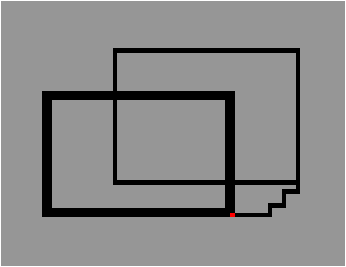
\includegraphics[scale=0.7]{drafts/book-ora017}}
	\caption{\label{fig:telecran}Telecran}
\end{figure}
